\documentclass[11.5pt]{sig-alternate} % sets document style to sig-alternate
% packages
% typesetting
%\usepackage{dirtytalk} % typset quotations easier (\say{stuff})
\usepackage{hanging} % hanging paragraphs
\usepackage[defaultlines=3,all]{nowidow} % avoid widows
\usepackage[pdfpagelabels=false]{hyperref} % produce hypertext links, includes backref and nameref
\usepackage{xurl} % defines url linebreaks, loads url package
\usepackage{microtype}
\usepackage{textgreek}
%\usepackage{textcomp}
%\newcommand{\texttildemid}{\raisebox{0.4ex}{\texttildelow}}
% layout
\usepackage{enumitem} % control layout of itemize, enumerate, description
\usepackage{fancyhdr} % control page headers and footers
\usepackage{float} % improved interface for floating objects
%\usepackage{multicol} % intermix single and multiple column pages
% language
\usepackage[utf8]{inputenc} % accept different input encodings
\usepackage[english]{babel} % multilanguage support
% misc
\usepackage{graphicx} % builds upon graphics package, \includegraphics
%\usepackage{lastpage} % reference number of pages
%\usepackage{comment} % exclude portions of text (?)
\usepackage{xcolor} % color extensions
\usepackage[backend=biber, style=apa]{biblatex} % sophisticated bibliographies % necessary for HTML to display author info and date on abstract page
\usepackage{csquotes} % advanced quotations, makes biblatex happy
\usepackage{authblk} % support for footnote style author/affiliation
% tables and figures
\usepackage{tabularray}
%\usepackage{array} % extend array and tabular environments
\usepackage{caption} % customize captions in figures and tables (rotating captions, sideways captions, etc)
%\usepackage{cuted} % allow mixing of \onecolumn and \twocolumn on same page
\usepackage{multirow} % create tabular cells spanning multiple rows
%\usepackage{subfigure} % deprecated, support for manipulation of small figures
%\usepackage{tabularx} % extension of tabular with column designator "x", creates paragraph-like column whose width automatically expands
%\usepackage{wrapfig} % allows figures or tables to have text wrapped around them
%\usepackage{booktabs} % better rules
% dummy text
%\usepackage{blindtext} % blind text dummy text
%\usepackage{kantlipsum} % Kant style dummy text
\usepackage{lipsum} %lorem ipsum dummy text
% other helpful packages may be booktabs, longtable, longtabu, microtype

\pagestyle{fancy} % sets pagestyle to fancy for fancy headers and footers

% header and footer
% modern way to set header image
\renewcommand{\headrulewidth}{0pt} % defines thickness of line under header
\renewcommand{\footrulewidth}{0pt} % defines thickness of line above header
\setlength\headheight{80.0pt} % sets height between top margin and header image, effectively moves page contents down
\addtolength{\textheight}{-80.0pt} % seems to affect the lower height. maybe only works properly if footer numbers enabled?
\fancyhf{}
\fancyhead[CE, CO]{
\includegraphics[width=\textwidth]{headerImage.png}}
% footer
%\fancyfoot[LE,LO]{Article Title Here \\ DOI: }% left footer article title and doi
%\fancyfoot[CE,CO]{{}} % center footer empty
%\fancyfoot[RE,RO]{\thepage} % right footer page numbers
%\pagenumbering{arabic} % arabic (1, 2, 3) numbering in footer

\hypersetup{colorlinks=true,urlcolor=blue} % sets link color to blue
\urlstyle{same} % sets url typeface to same as rest of text

% set caption and figure to italics, label bold, left align captions, does not transfer to HTML
\captionsetup{labelfont=bf, font={large, it}, justification=raggedright, singlelinecheck=false}
\renewcommand\theContinuedFloat{\alph{ContinuedFloat}}

%this next bit is confusing, but essentially changes the width of the abstract. Seems to have been copied from this https://tex.stackexchange.com/questions/151583/how-to-adjust-the-width-of-abstract
\let\oldabstract\abstract
\let\oldendabstract\endabstract
\makeatletter %changes @ catcode to enable modification (in parsep)
\renewenvironment{abstract} %alters the abstract environment
{\renewenvironment{quotation}%
               {\list{}{\addtolength{\leftmargin}{1em} % change this value to add or remove length to the the default ?
                        \listparindent 1.5em%
                        \itemindent    \listparindent%
                        \rightmargin   \leftmargin%
                        \parsep        \z@ \@plus\p@}%
                \item\relax}%
               {\endlist}%
\oldabstract}
{\oldendabstract}
\makeatother %changes @ catcode to disable modification

% checks
% italics
% links
% dashes
% tildes
\begin{document}

\title{Ex Ovo Omnia}

\author[1]{\large \color{blue}Todd Pagano}

\affil[1]{Rochester Institute of Technology/ National Technical Institute for the Deaf}

\toappear{}
%% ABSTRACT
\maketitle
\begin{@twocolumnfalse} 
\begin{abstract}
\item 
\textit{One of history’s most diverse thinkers metaphorically depicted humanity’s dangerous reliance on nonrenewable energy resources as an unborn chick in an egg. American philosopher, poet, scientist, and mathematician, Buckminster Fuller, described the nutrients in an egg as the temporary and extinguishable support required for the development of an unhatched chick. Once the nutrients are depleted, the chick must break from its shell and cultivate its own mechanism for survival. Symbolically, he explained that the human population must view the use of earth’s finite resources as the nutriment in an egg that can be provisionally relied upon in order to provide the necessary time and energy required for mankind to establish alternative energy sources for a sustainable future. I use Bucky’s metaphor to describe my own teaching philosophy; the role of the educator as that of a facilitator, or provider of the “egg”. Using this mindset and a variety of learning modalities in my classroom, I am hopeful that at the end of the educational process, my students emerge from their “shells” with the necessary skills to be renewable sources of learning unto themselves.}
\\ \\

\end{abstract}
\end{@twocolumnfalse}

%% AUTHOR INFORMATION

\textbf{*Corresponding Author, Todd Pagano}\\
\href{mailto:tepnts@rit.edu}{(tepnts@rit.edu)} \\
\textit{Submitted  Aug 15 2014 }\\
\textit{Accepted  Aug 15 2014} \\
\textit{Published online Aug 15 2014} \\
\textit{DOI: 10.14448/jsesd.05.0005} \\
\pagebreak
\clearpage
\begin{large}

Teaching, like the structure of any metaphor, has a \textit{topic} and a \textit{vehicle}. The \textit{topic} is the intended knowledge that the instructor wishes to disseminate. The \textit{vehicle} is the mechanism of cultivating the intended \textit{topic}. Both should be continually addressed in lesson planning through self-reflection and assessment.

\begin{figure}[h]
    \centering
    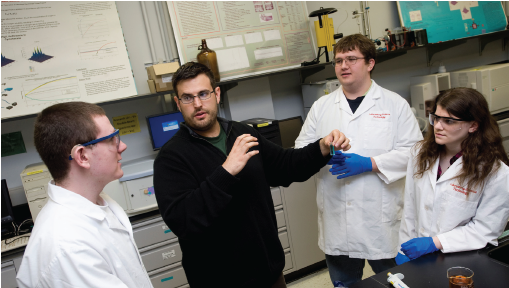
\includegraphics[width=1\linewidth]{fig2.png}
\end{figure}

\textit{The Topics:} In concert with RIT/NTID’s Mission Statement, it is imperative to foster learning in the content area without skewing the development of lifelong skills that will help students thrive in the professional community. Professors should facilitate interdisciplinary and general learning, not merely disseminate content-specific information. For example, deaf and hard-of-hearing students in RIT/NTID’s Laboratory Science Technology program not only require the crucial knowledge in the field of chemical testing (i.e. instrumentation, gravimetric/volumetric analyses, etc.), but also critical thinking proficiencies, general science literacy, ethical decision making, global community awareness, and self-advocacy/workplace survival skills.

\textit{The Vehicles:} Useful mechanisms for conveying information include reaching the target audience at the appropriate level while being cognizant of different learning styles, making the material interesting and relevant, and using innovative pedagogical tools. Effective teachers are versed in the scholarship of their field and also have the ability to teach the subject at a suitable level for the identified group of learners. Flexibility in one’s presentation, and an understanding of various learning modes, are paramount to stimulating students who often enter the science classroom/teaching laboratory not truly understanding the subject, how it relates to their lives/interests, or how it will benefit them beyond merely fulfilling degree requirements or prerequisites. It is imperative for instructors to break down these barriers in order to give students an appreciation for the course material, an intimate relationship to the course, and direction. By incorporating real-world/contemporary issues, historical perspectives, and interdisciplinary topics, educators can better express the importance of the course, facilitate student learning, and make the subject captivating/enjoyable/memorable. The use of a variety of pedagogical tools; like supportive technology, inquiry-based and active learning, and involvement in scholarly research can further promote student success by assisting in the transformation of abstract ideas into applicable concepts.

\begin{quote}
\underline{RIT/NTID's Mission Statement}

``To provide deaf and hard-of-hearing students with outstanding state-of-the-art technical and professional programs... prepare them to live and work in the mainstream of a rapidly changing global community and enhance their lifelong learning.''
\end{quote}

Given proper nutriment, a \textit{chick} hatches from the \textit{eggshell} to become a reproductive chicken and a student develops into a knowledgeable \textit{lifelong learner}. Keeping with this metaphor, a change in perspective on the age-old question is put forth: \textit{“Which came first- the teacher or the student?”} I believe that teaching is reciprocal; thus, a teacher is a student. In the context of the shared mission of student success by the teacher and the student, instructors should be willing to learn, not only by keeping current in their field, but also by learning from their students. Acquiring, modifying, and improving teaching skills are dynamic processes that can be continually developed through feedback from students and peers, as well as through comprehensive self-reflection.

\textit{…ex ovo omnia (all from the egg)…}

\section*{BIOGRAPHICAL STATEMENT}

Dr. Todd Pagano is an Associate Professor of Science \& Mathematics at Rochester Institute of Technology and Director of the National Technical Institute for  the Deaf’s Laboratory Science Technology program; a oneof-kind program in the world (i.e., a postsecondary chemical technology program for deaf and hard-of-hearing students). During his career at RIT/NTID, he has led the design and implementation of the LST program, set-up a state-of-the-art instrumentation laboratory, architected the new degree program, and helped to place a large number of deaf and hard-of-hearing individuals into careers in the chemical sciences. He has been honored as a recipient of several awards, including: RIT’s Richard \& Virginia Eisenhart Award for Excellence in Teaching, Dawan L. Albritton Faculty Humanitarian Award, NTID’s Faculty Research Scholar Award, and the American Chemical Society’s (ACS) Stanley C. Israel Medal for Advancing Diversity in the Chemical Sciences. He leads several chemical and pedagogical research projects and is a Fellow of the ACS.

\end{large}

\end{document}
